
\subsection{Protocol and statement of results}


Throughout this section we 
let $\Sigma=\{X,Y,Z,F,G\}$, and let $m=\Theta(n+t)$ be chosen 
large enough so that each symbol in $\Sigma$ appears at least $n+t$ times in a uniform random $W\in\Sigma^m$, with probability close to $1$.
Let $\mu({W})$ denote the probability that a player receives input ${W}$ while playing $\rigid(\Sigma,m)$ (recall that both players have the same marginals in $\rigid$). Let $\mu({W}'|{W})$ denote the probability that one player receives ${W}'$ given that the other player receives~${W}$. 

The full protocols are presented in Figure \ref{fig:dogwalker-protocol-V} (verifier's point of view), Figure \ref{fig:dogwalker-protocol-PV} ($\pv$'s point of view) and Figure \ref{fig:dogwalker-protocol-PP} ($\pp$'s point of view). The protocol has two 
types of runs: 
EPR and Rigidity. Within an EPR run are three 
types of sub-runs: 
Computation sub-run, $X$-test sub-run, and $Z$-test sub-run. We will generally think of $X$- and $Z$-test sub-runs as one sub-run type (Test sub-run). Within a Rigidity run are two types of sub-runs: Tomography sub-run, which should be thought of as the Rigidity version of the EPR-Computation run; and Clifford sub-run, which should be thought of as the Rigidity version of the EPR-Test run. With some probability $p_1$, $\ver$ runs a Rigidity run, Clifford sub-run; with some probability $p_2$, $\ver$ runs an EPR run, Test sub-run; with some probability $p_3$, $\ver$ runs an EPR run, Computation sub-run; and with probability $p_4=1-p_1-p_2-p_3$, $\ver$ runs a Rigidity run, Tomography sub-run. This structure is illustrated in Figure~\ref{fig:DogWalkerFig}. We call this the Dog-Walker Protocol with parameters $(p_1,p_2,p_3,p_4)$.

 \begin{figure}[ht]
    \centering{
    \begin{tikzpicture}
%    \draw (-7.8,-4.65)--(7.8,-4.65);
    
    % ROOT
    \node at (0,0) {\begin{minipage}{2in}\centering
        {\Large \underline{Dog Walker}}\\ Fig.~\ref{fig:dogwalker-protocol-PP}, Fig.~\ref{fig:dogwalker-protocol-PV}, and Fig.~\ref{fig:dogwalker-protocol-V}
    \end{minipage}};
        % L-CHILD (Rigidity)
        \node at (-3.25,-1) {$p_1+p_4$};
        \draw (0,-.5)--(-5,-1.75); 
        \node at (-5,-2.5) {\begin{minipage}{1.5in}\centering
            \underline{Rigidity Run}\\
            \RaggedRight
            Ensure $\pv$ behaves honestly
        \end{minipage}};
        
            % L-CHILD -- L-CHILD (Computation/Tomography)
            \node at (-6,-3.7) {$\frac{p_4}{p_1+p_4}$};
            \draw (-5,-3) -- (-5.85,-4.5);
            \node at (-5.85,-6.5) {\begin{minipage}{1.4in}\centering
                \underline{Computation Sub-run}\\ \underline{(Tomography)}\\
                \RaggedRight
                Ensure $\pv$ reports correct measurements when he gets to choose measurement to perform using $\textsc{tom}$ (Fig.~\ref{fig:tomography-test})
            \end{minipage}};
            
            % L-CHILD -- R-CHILD (Test/Clifford)
            \node at (-2.5,-3.7) {$\frac{p_1}{p_1+p_4}$};
            \draw (-5,-3) -- (-1.95,-4.5);
            \node at (-1.95,-5.775) {\begin{minipage}{1.4in}\centering
                \underline{Test Sub-run}\\ \underline{(Clifford)}\\
                \RaggedRight
                Ensure $\pv$ applies correct gates using $\textsc{rigid}$ (Fig.~\ref{fig:rigid})
            \end{minipage}};
        % R-CHILD (EPR)
        \node at (3.5,-1) {$p_2+p_3$};
        \draw (0,-.5)--(5,-1.75);
        \node at (5,-2.5) {\begin{minipage}{1.75in}\centering
            \underline{EPR Run}\\
            \RaggedRight
            $\pv$ uses EPR Protocol to delegate computation to $\pp$
        \end{minipage}};
        
            % R-CHILD -- L-CHILD (Computation)
            \node at (2.8,-3.7) {$\frac{p_2}{p_2+p_3}$};
            \draw (5,-3.2) -- (1.95,-4.5);
            \node at (1.95,-4.82)
            {\begin{minipage}{1.4in}\centering
                \underline{Test Sub-run}
            \end{minipage}};
                % R-CHILD -- R-CHILD -- L-CHILD (X-test)
                \node at (.6,-6) {$\sfrac{1}{2}$};
                \draw (1.95,-5.1) -- (0,-7);
                \node at (0,-8.5)
                {\begin{minipage}{1.4in}\centering
                    \underline{$X$-Test}\\           \RaggedRight
                    Ensure $\pp$ returns correctly measured bits, except for those returned on odd $\sf T$ gate gadgets
                \end{minipage}};
                % R-CHILD -- R-CHILD -- R-CHILD (Z-test)
                \node at (3.2,-6) {$\sfrac{1}{2}$};
                \draw (1.95,-5.1) -- (3.9,-7);
                \node at (3.9,-8.25)
                {\begin{minipage}{1.4in}\centering
                    \underline{$Z$-Test}\\           \RaggedRight
                    Ensure $\pp$ returns correctly measured bits on odd $\sf T$ gate gadgets
                \end{minipage}};
            % R-CHILD -- R-CHILD (Test)
            \node at (6,-3.7) {$\frac{p_3}{p_2+p_3}$};
            \draw (5,-3.2) -- (5.85,-4.5);            
            \node at (5.85,-5.05)
            {\begin{minipage}{1.4in}\centering
                \underline{Computation Sub-run}\\           \RaggedRight
                Run the computation
            \end{minipage}};
    \end{tikzpicture}}
    \caption{The structure of the Dog-Walker Protocol. We illustrate the structure of different runs, sub-runs, and games/tests, letting probabilities label branches.}
    \label{fig:DogWalkerFig}
\end{figure}



The following theorem states the guarantees of the Dog-Walker Protocol.

\begin{theorem}\label{thm:dog-walker}
There exist constants $p_1$, $p_2$, $p_3$, $p_4=1-p_1-p_2-p_3$, and $\Delta>0$ such that the following hold of the Dog-Walker Protocol with parameters $(p_1,p_2,p_3,p_4)$, when executed on input $(Q,\ket{\vec{x}})$.
\begin{itemize}
\item (Completeness: ) Suppose that $\norm{\Pi_0Q\ket{\vec{x}}}^2\geq 2/3$. Then
  there is a strategy for $\pv$ and $\pp$ that is accepted with probability at
    least $p_{\mathrm{compl}}=p_1(1-e^{-\Omega(n+t)})+p_2+\frac{2}{3}p_3 +
    p_4$. 
\item (Soundness: ) Suppose that $\norm{\Pi_0Q\ket{\vec{x}}}^2\leq 1/3$. Then any strategy for $\pv$ and $\pp$ is accepted with probability at most $p_{\mathrm{sound}}=p_{\mathrm{compl}}-\Delta$. 
\end{itemize}
\end{theorem}
\noindent The proof of completeness is given in Lemma \ref{lem:dogwalker-completeness}, and proof of soundness is given in Lemma \ref{lem:dogwalker-soundness}. 

%----------------%
\begin{figure}[H]
\rule[1ex]{\textwidth}{0.5pt}
\vspace{-20pt}
\justify
1. Select a run type \textbf{EPR} or \textbf{Rigidity}, and disjoint sets $N,T^0,T^1\subset \{1,\ldots,m\}$ of sizes $n$, $t_0$ and $t-t_0$.  
\begin{description}
\item[EPR] Choose $\vec{z}$ uniformly at random from $\{0,1\}^t$ and send it, along with $N$, $T^0$ and $T^1$, to $\pp$. Receive measurement outcomes $\vec{c}\in\{0,1\}^t$ and $c_f\in\{0,1\}$ from $\pp$.
\item[Rigidity] Choose $W'$ according to $\mu(\cdot)$ and send it to $\pp$. Receive $\vec{e}'\in \{0,1\}^m$ from $\pp$. 
\end{description}
2. Select a sub-run type at random from \textbf{Computation}, \textbf{X Test} or \textbf{Z Test}. 
\begin{description}
\item[Computation] Based on whether it's an \text{EPR} or a \text{Rigidity} Run:
	\begin{description}
	\item[EPR]
		\begin{enumerate}
		\item[(i)] Send $\vec{x}$, $\vec{z}$, $\vec{c}$ and sets $N$, $T^0$ and $T^1$ to $\pv$, and receive measurement outcomes $\vec{a},\vec{b}\in \{0,1\}^n$ and $\vec{e}\in\{0,1\}^t$.
		\item[(ii)] Apply the update rules from Table \ref{tab:EPR-key-updates} gate-by-gate to obtain the final $\sf X$ key for the output wire $a_f'$. If $c_f+a_f'\neq 0$, $\sf reject$. 
		\end{enumerate}
	\item[Rigidity (Tomography)]
		\begin{enumerate}
		\item[(i)] Choose uniform random strings $\vec{c},\vec{z}\in\{0,1\}^t$, $\vec{x} \in \{0,1\}^n$ 
		to send to $\pv$, along with $N$ and $T$, and receive measurement outcomes $\vec{d}\in \{0,1\}^n$ and $\vec{e}\in\{0,1\}^t$. 
		\item[(ii)]
		From $\vec{x}$, $\vec{c}$, $\vec{z}$, $\vec{d}$, and $\vec{e}$, determine the adaptive measurements $W\in\Sigma^{n+t}$ that $V_{EPR}^0$ would have performed (based on Figure \ref{fig:original-protocol-VEPRr}), and $\sf reject$ if the input-output pairs $(W',\vec{e}')$ and $(N\cup T,(W,\vec{e}))$ do not satisfy the winning criterion for $\tom(\Sigma,n+t,m)$.
		\end{enumerate}
	\end{description}
\item[$X$-Test] Based on whether it's an \text{EPR} or a \text{Rigidity} Run:
\begin{description}
	\item[EPR] 
	\begin{enumerate}
		\item[(i)] Choose $W\in\Sigma^m$ uniformly at random among all strings satisfying: $W_i=Z$ for all $i\in N$; $W_i=Z$ for all $i\in T^0$; and $W_i\in\{X,Y\}$ for all $i\in T^1$. Send $W$ to $\pv$ and receive measurement results $\vec{e}\in\{0,1\}^m$. Let $(\vec{a},\vec{b})=(\vec{e}_N,0^n)$. 
		\item[(ii)] Apply update rules from Table \ref{tab:EPR-key-updates} gate-by-gate to obtain $\forall i\in [t]$ the $\sf X$ key before the $i$-th $\sf T$ gate is applied, $a_i'$, and the final $\sf X$ key for the output wire, $a_f'$. 
If $\exists i$ s.t.\ the $i$-th $\sf T$ gate is even and $c_i\neq a_i'+e_i$, $\sf reject$. If $c_f+a_f'\neq 0$, $\sf reject$. 
	\end{enumerate}
	\item[Rigidity (Clifford)] Choose ${W}$ according to the marginal conditioned on ${W}'$, $\mu(\cdot|{W}')$. 
	Send ${W}$ to $\pv$ and receive $\vec{e}\in\{0,1\}^m$. Reject if   $({W}',\vec{e}',{W},\vec{e})$ doesn't win $\rigid(\Sigma,m)$. 
\end{description}

\item[$Z$-Test] Based on whether it's an \text{EPR} or a \text{Rigidity} Run:
\begin{description}
	\item[EPR] 
	\begin{enumerate}
		\item[(i)] Choose $W\in\Sigma^m$ uniformly at random among all strings satisfying: $W_i=X$ for all $i\in N$; $W_i\in\{X,Y\}$ for all $i\in T^0$; and $W_i=Z$ for all $i\in T^1$. Send $W$ to $\pv$ and receive measurement results $\vec{e}\in\{0,1\}^m$. Let $(\vec{a},\vec{b})=(0^n,\vec{e}_N)$.
		\item[(ii)] Apply update rules from Table \ref{tab:EPR-key-updates} gate-by-gate to obtain $\forall i\in [t]$, the $\sf X$ key before the $i$-th $\sf T$ gate is applied, $a_i'$. 
If $\exists i$ s.t.\ the $i$-th $\sf T$ gate is odd and $c_i\neq a_i'+e_i$, $\sf reject$. 
	\end{enumerate}
	\item[Rigidity (Clifford)] Identical to $X$-Test case.
\end{description}
\end{description}
\rule[2ex]{\textwidth}{0.5pt}\vspace{-.5cm}
\caption{The Dog-Walker Protocol: Verifier's point of view.}\label{fig:dogwalker-protocol-V}
\end{figure}




\begin{figure}[H]
\rule[1ex]{\textwidth}{0.5pt}
\vspace{-20pt}
\begin{enumerate}
  \item If $\pv$ receives a question ${W}$ from $\ver$ (he is playing $\rigid$ or an $X$- or $Z$-Test Run):
\begin{enumerate}
     \item[]  Measure the $m$ qubits in the observable indicated by $W$ --- for example, if $W\in \Sigma^m$, for $i\in \{1,\ldots,m\}$, measure the $i$-th qubit in the basis indicated by $W_i$ --- and report the outcomes $\vec{e}$ to $\ver$.
\end{enumerate}

  \item If $\pv$ receives $\vec{x}$, $\vec{z}$, $\vec{c}$ and sets $N$, $T^0$ and $T^1$ from $\ver$ (he is playing $\tom$ or a Computation Run):
\begin{enumerate}
	\item[] Run the procedure $V_{EPR}^0$ from Figure \ref{fig:original-protocol-VEPRr} on input $\vec{x}$, $\vec{c}$, $\vec{z}$, the $n$ qubits in $N$, and the $t$ qubits in $T^0\cup T^1$. Report the outputs  $\vec{d}$ and $\vec{e}$ of $V_{EPR}^0$ to $\ver$.
\end{enumerate}
\end{enumerate}
\rule[2ex]{\textwidth}{0.5pt}\vspace{-.5cm}
\caption{The Dog-Walker Protocol: Honest strategy for $\pv$.}\label{fig:dogwalker-protocol-PV}
\end{figure}

\begin{figure}[H]
\rule[1ex]{\textwidth}{0.5pt}
\vspace{-20pt}
\begin{enumerate}
  \item If $\pp$ receives a question ${W}'$ from $\ver$ (he is playing $\tom$ or $\rigid$):
\begin{enumerate}
     \item[]  Measure the $m$ qubits in the observable indicated by $W'$ --- for example, if $W'\in\Sigma^m$, for $i\in \{1,\ldots,m\}$, measure the $i$-th qubit in the basis indicated by $W_i'$ --- and report
       the outcomes $\vec{e}'$ to~$\ver$.
\end{enumerate}
\item If $\pp$ receives $\vec{z}$, and sets $N$, $T^0$ and $T^1$ from $\ver$ (he is playing the role of $P_{EPR}$ from the EPR Protocol):
\begin{enumerate}
     \item[] Run the prover $P_{EPR}$ from Figure \ref{fig:original-protocol-PEPR} on input $\vec{z}$, the $n$ qubits in $N$, and the $t$ qubits in $T^0\cup T^1$.
     Report the outputs $\vec{c}\in\{0,1\}^t$ and $c_f\in\{0,1\}$ of $P_{EPR}$  to $\ver$. 
\end{enumerate}
\end{enumerate}
\rule[2ex]{\textwidth}{0.5pt}\vspace{-.5cm}
\caption{The Dog-Walker Protocol: Honest strategy for $\pp$.}\label{fig:dogwalker-protocol-PP}
\end{figure}


\subsection{Completeness}

\begin{lemma}\label{lem:dogwalker-completeness}
Suppose $\ver$ executes the Dog-Walker Protocol with parameters $(p_1,p_2,p_3,p_4)$.
There is a strategy for the provers such that, on any input $(Q,\ket{\vec{x}})$
  such that $\norm{\Pi_0 Q\ket{\vec{x}}}^2\geq \frac{2}{3}$, $\ver$ accepts with
  probability at least
  $p_{\mathrm{compl}}=p_1(1-\delta_c)+p_2+\frac{2}{3}p_3+p_4$, for some $\delta_c = e^{-\Omega(n+t)}$.
\end{lemma}

\begin{proof}
The provers $\pv$ and $\pp$ play the strategy described in Figures
  \ref{fig:dogwalker-protocol-PV} and \ref{fig:dogwalker-protocol-PP}
  respectively. In the Rigidity-Tomography run, the verification performed by
  $\ver$ amounts to playing $\tom(\Sigma,n+t,m)$ with the provers (with an extra
  constraint on the output $W$ of $\pv$ that is always satisfied by the honest
  strategy). This game has perfect
  completeness, which makes the $\ver$
  accept with probability $1$ in the Rigidity-Tomography run.
  In the Rigidity-Clifford run, $\ver$ plays $\rigid(\Sigma,m)$
  with the provers. The game
  has completeness at least $1-\delta_c$ for some $\delta_c=e^{-\Omega(n+t)}$,
  since $m=\Omega(n+t)$, therefore their success probability in this run is
  at least $1-\delta_c$.

In the EPR run, the provers are exactly carrying out the EPR Protocol, with $\ver$ using $\pv$ to run $V_{EPR}^r$, and $\pp$ playing the role of $P_{EPR}$. Thus, test runs result in acceptance with probability $1$, and the computation run results in acceptance with probability $\norm{\Pi_0 Q\ket{\vec{x}}}^2$, by Theorem \ref{thm:EPR-correctness}. 
\end{proof}


\subsection{Soundness}

Figure~\ref{fig:full-dog-walker} summarizes the high-level structure of the soundness analysis. Intuitively, our ultimate goal is to argue that both provers either apply the correct operations in EPR-Computation runs, or are rejected with constant probability. This will be achieved by employing a form of ``hybrid argument'' whereby it is argued that the provers, if they are not caught, must be using the honest strategies described in Figure~\ref{fig:dogwalker-protocol-PP} and Figure~\ref{fig:dogwalker-protocol-PV} in the different types of runs considered in the protocol. Towards this, we divide the run types into the following four scenarios:
\begin{enumerate}
\item Rigidity-Clifford: The run type is \textbf{Rigidity} and the sub-run type is either \textbf{$X$-Test} or \textbf{$Z$-Test}. (When the provers are honest) $\pv$ behaves as in Item 1 of Figure \ref{fig:dogwalker-protocol-PV}, and $\pp$ behaves as in Item 1 of Figure \ref{fig:dogwalker-protocol-PP}. 
\item EPR-Test: The run type is \textbf{EPR} and the sub-run type is either \textbf{$X$-Test} or \textbf{$Z$-Test}. $\pv$ behaves as  in Item 1 of Figure \ref{fig:dogwalker-protocol-PV}, and $\pp$ behaves as in Item 2 of Figure \ref{fig:dogwalker-protocol-PP}. 
\item EPR-Computation: The run type is \textbf{EPR} and the sub-run type is \textbf{Computation}. $\pv$ behaves as in Item 2 of Figure \ref{fig:dogwalker-protocol-PV}, and $\pp$ behaves as in Item 2 of Figure \ref{fig:dogwalker-protocol-PP}. 
\item Rigidity-Tomography: The run type is \textbf{Rigidity} and the sub-run type is \textbf{Computation}. $\pv$ behaves as in Item 2 of Figure \ref{fig:dogwalker-protocol-PV}, and $\pp$ behaves as in Item 1 of Figure \ref{fig:dogwalker-protocol-PP}. 
\end{enumerate}
Examining Figure \ref{fig:dogwalker-protocol-V}, we can see the following. In the Rigidity-Clifford scenario, the verifier is precisely playing the game $\rigid$ with the provers, as the provers receive questions $W'$ and $W$ distributed according to $\mu(\cdot,\cdot)$, the distribution of questions for $\rigid(\Sigma,m)$; their answers are tested against the winning conditions of $\rigid(\Sigma,m)$. In the Rigidity-Tomography scenario, the verifier plays a variant of the game $\tom$ with the provers, in which $\pv$'s choice of observable $W$ is uniquely determined by his inputs $\vec{x}$, $\vec{c}$ and $\vec{z}$: it should match the observable implemented by $V_{EPR}^0$ on these inputs. In EPR runs, $\pv$ plays the part of $V_{EPR}^r$ from the EPR Protocol, and $\pp$ plays the part of $P_{EPR}$. The EPR-Test scenario corresponds to $X$- and $Z$-tests from the EPR Protocol, whereas the EPR-Computation scenario corresponds to computation runs from the EPR Protocol.

\begin{figure}[H]
\centering
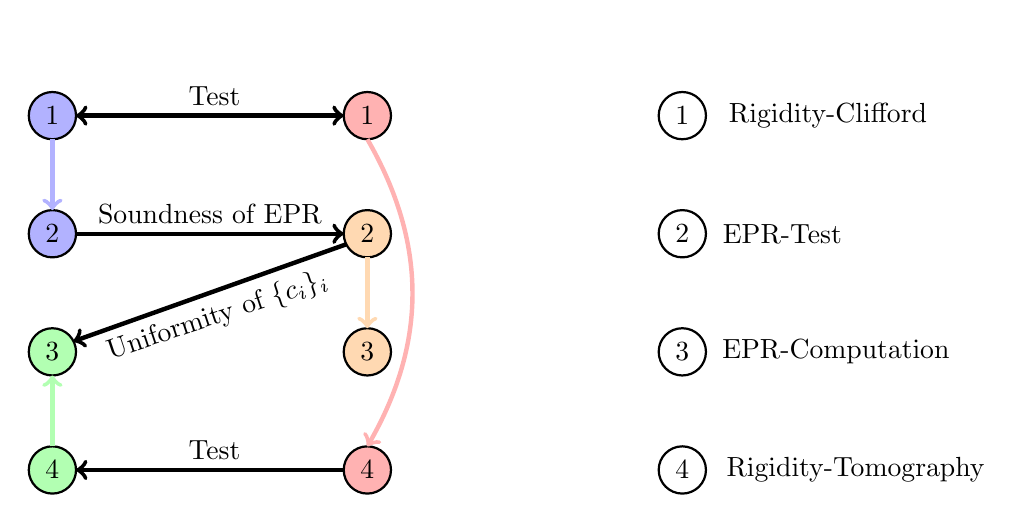
\begin{tikzpicture}
\filldraw[thick, fill=blue!30!white] (0,6) circle (.3);
\filldraw[thick, fill=blue!30!white] (0,4.5) circle (.3);
\filldraw[thick, fill=green!30!white] (0,3) circle (.3);
\filldraw[thick, fill=green!30!white] (0,1.5) circle (.3);

\filldraw[thick, fill=red!30!white] (4,6) circle (.3);
\filldraw[thick, fill=orange!30!white] (4,4.5) circle (.3);
\filldraw[thick, fill=orange!30!white] (4,3) circle (.3);
\filldraw[thick, fill=red!30!white] (4,1.5) circle (.3);

\node at (0,6) {1};
\node at (4,6) {1};
\node at (0,4.5) {2};
\node at (4,4.5) {2};
\node at (0,3) {3};
\node at (4,3) {3};
\node at (0,1.5) {4};
\node at (4,1.5) {4};

\draw[ultra thick, ->, blue!30!white] (0,5.7)--(0,4.8);
\draw[ultra thick, ->, green!30!white] (0,1.8)--(0,2.7);
\path[ultra thick, ->, orange!30!white] (4,4.2) edge (4,3.3);
\path[ultra thick, ->, red!30!white] (4,5.7) edge[bend left] (4,1.8);

\draw[ultra thick, <->] (.3,6)--(3.7,6);
\draw[ultra thick, ->] (.3,4.5)--(3.7,4.5);
\draw[ultra thick, <-] (.268,3.134)--(3.732,4.366);
\draw[ultra thick, <-] (.3,1.5)--(3.7,1.5);

\node at (2,6.25) {$\rigid$ Test};
\node at (2,4.75) {Soundness of EPR};
\node [rotate=18.5] at (2.1,3.45) {Uniformity of $\{c_i\}_i$};
\node at (2,1.75) {$\tom$ Test};

\draw[thick] (8,6) circle (.3);
\node at (8,6) {1};
\node at (9.85,6) {Rigidity-Clifford};

\draw[thick] (8,4.5) circle (.3);
\node at (8,4.5) {2};
\node at (9.27,4.5) {EPR-Test};

\draw[thick] (8,3) circle (.3);
\node at (8,3) {3};
\node at (9.95,3) {EPR-Computation};

\draw[thick] (8,1.5) circle (.3);
\node at (8,1.5) {4};
\node at (10.2,1.5) {Rigidity-Tomography};

\node at (0,7) {\pv};
\node at (4,7) {\pp};

%\draw (1.8,5.9) rectangle (2.2,5.5);
%\node at (2,5.7) {\small i};

%\draw (-.5,5.05) rectangle (-.1,5.45);
%\node at (-.3,5.25) {\small ii};

%\draw (4.65,3.55) rectangle (5.05,3.95);
%\node at (4.85,3.75) {\small iii};

%\draw (1.8,4.0) rectangle (2.2,4.4);
%\node at (2,4.2) {\small iv};

%\draw (4.05,3.95) rectangle (4.45,3.55);
%\node at (4.25,3.75) {\small vii};

%\draw (1.2,3.95) rectangle (.8,3.55);
%\node at (1,3.75) {\small iv};

%\draw (1.8,1.05) rectangle (2.2,1.45);
%\node at (2,1.25) {\small v};

%\draw (-.5,2.0) rectangle (-.1,2.4);
%\node at (-.3,2.2) {\small vi};


\end{tikzpicture}
\caption{Overview of the soundness of the Dog-Walker Protocol}\label{fig:full-dog-walker}
\end{figure}




\noindent The structure of the proof is as follows (see also Figure~\ref{fig:full-dog-walker}):
\begin{enumerate}
\item[(i)] By the game $\rigid$, in the Rigidity-Clifford runs, both $\pp$ and $\pv$ must be honest, or they would lose the game.
\item[(ii)] Since $\pv$ can't distinguish between Rigidity-Clifford and EPR-Test (both are Figure \ref{fig:dogwalker-protocol-PV} Item 1 from his perspective, and the input distributions, while not identical, have total variation distance $1 - \eta$, for some constant $\eta > 0$), $\pv$ must be honest in the EPR-Test runs, by (i). 
\item[(iii)] Since $\pp$ can't distinguish between Rigidity-Clifford and Rigidity-Tomography (both are Figure~\ref{fig:dogwalker-protocol-PP} Item 1 from his perspective), $\pp$ must be honest in the Rigidity-Tomography runs, by~(i). 
\item[(iv)] Since $\pv$ is honest in EPR-Test runs by (ii), $\pp$ must be honest in EPR-Test runs or he will get caught, but in particular, he must output values $\{c_i\}_{i\in [t]}$ that are uniform random and independent of $\vec{z}$. Since $\pp$ can't distinguish between EPR-Test and EPR-Computation runs, this is also true in EPR-Computation runs, when the verifier sends the values $\{c_i\}_i$ to $\pv$. 
\item[(v)] $\pv$ must be honest in Rigidity-Tomography runs, or the provers would lose the game $\tom$.
\item[(vi)] Since $\pv$ can't distinguish between Rigidity-Tomography runs and EPR-Computation runs (both are Figure \ref{fig:dogwalker-protocol-PV} Item 2 from his perspective), $\pv$ must be honest in EPR-Computation runs, by~(v), and his input distribution to both runs has total variation distance $1 - \eta'$, for some constant $\eta' > 0$, by (iv).
\item[(vii)] Since $\pv$ is honest in EPR-Test runs by (ii), and EPR-Computation runs by (vi), the combined behavior of $\ver$ and $\pv$ in the EPR runs is that of $V_{EPR}$ in the EPR Protocol, so
by the soundness of the EPR Protocol, $\pp$ must be honest in EPR-Computation runs, or get caught in the EPR-Test runs with high probability.
\end{enumerate}

 The following lemma establishes (i), (ii) and (iii). 

\begin{lemma}\label{lem:PV-2-PP-4}
Suppose the verifier executes the Dog-Walker Protocol 
with provers $(\pv^*,\pp^*)$ such that the provers are accepted with probability $q_1\geq 1-\eps$ in the Rigidity-Clifford Run, $q_2$ in the EPR-Test Run, $q_3$ in the EPR-Computation Run, and $q_4$ in the Rigidity-Tomography Run. Then there exist provers $(\pv',\pp')$ such that:
\begin{itemize}[nolistsep]
\item $\pv'$ and $\pp'$ both apply the honest strategy in the Rigidity-Clifford runs, $\pv'$ applies the honest strategy in the EPR-Test runs, and $\pp'$ applies the honest strategy in the Rigidity-Tomography runs; in particular, the state shared by the provers at the beginning of the protocol is a tensor product of the honest state consisting of $m$ shared EPR pairs and an arbitrary shared ancilla;
\item The provers are accepted with probability $q_2'=q_2-O(\mathrm{poly}(\eps))$ in the EPR-Test Run, $q_3'=q_3$ in the EPR-Computation Run, and $q_4'=q_4-O(\mathrm{poly}(\eps))$ in the Rigidity-Tomography Run. 
\end{itemize}
\end{lemma}

\begin{proof}
Using a similar argument as in Lemma~\ref{soundlemma}, the strategy of $\pv^*$ in
Rigidity-Clifford runs, which is also his strategy in EPR-Test runs (Figure \ref{fig:dogwalker-protocol-PV} Item 1); and the strategy of $\pp^*$ in Rigidity-Clifford runs, which is also his strategy in Rigidity-Tomography runs (Figure \ref{fig:dogwalker-protocol-PP} Item 1);
 can both be replaced with the honest strategies. Since the distribution of inputs to $\pp^*$ in the Rigidity-Tomography runs and Rigidity-Clifford runs is the same, the success probability in the Rigidity-Tomography runs is changed by at most $O(\mathrm{poly}(\eps))$ by using the honest strategy. 
On the other hand, $\pv^*$'s input distribution in EPR-Test runs is uniform on $\Sigma^m$, whereas his distribution in Rigidity-Clifford runs is given by $\mu$. However, from the description of the test $\rigid$ it is clear that for all $W\in\Sigma^m$, $\mu(W)\geq \frac{1}{c|\Sigma|^m}$ for some constant $c>1$, thus the total variation distance between the two distributions is at most $1-\frac{1}{c}$. Thus, replacing $\pv^*$ with the honest strategy in the EPR-Test  runs will change the success probability by at most  $O(\mathrm{poly}(\eps))$. 

Finally, since the provers' strategy in the EPR-Computation run has not changed, the
  acceptance probability in it remains unchanged.
\end{proof}

Next, we will show that whenever $\pv^*$ is honest in the EPR-Test runs this forces $\pp^*$ to output (close to) uniformly random $\{c_i\}_{i\in [t]}$ that are independent of the run type, even given $\vec{z}$. This will allow us to verify that $\pp^*$ is unable to signal to $\pv^*$ whether the run is an EPR Run in the EPR-Computation run, when $\pv^*$ is sent $\vec{z}$ and $\vec{c}$. This establishes (iv). 


\begin{lemma}\label{lem:ci-unif}
Suppose the verifier executes the Dog-Walker Protocol with provers $(\pv^*,\pp^*)$ such that the initial shared state of the provers consists of $m$ shared EPR pairs, together with an arbitrary shared auxiliary state; $\pv^*$ plays the honest strategy in the EPR-Test runs; the provers are accepted with probability $q_1$ in the Rigidity-Clifford Run, $q_2 = 1-\eps'$ in the EPR-Test Run, $q_3$ in the EPR-Computation Run, and $q_4$ in the Rigidity-Tomography Run. Then the input $(\vec{c},\vec{z})$ given by the verifier to $\pv^*$ in the EPR-Computation runs has a distribution that is within $O(\eps')$ total variation distance of uniform on $\{0,1\}^t\times\{0,1\}^t$. 
\end{lemma}

\begin{proof}
Let $a_i'$ denote the $\sf X$ key of the wire to which the $i$-th $\sf T$ gate is applied, just before the $i$-th $\sf T$ gate is applied, and let $D_i$ be a random variable defined as follows. If the $i$-th $\sf T$ gate is even, let $D_i=e_i+a_i'$, where we interpret $e_i$ and $a_i'$ as the random variables representing the measurement result and key $\ver$ would get if she chooses to execute an $X$-Test run. If the $i$-th $\sf T$ gate is odd, let $D_i=e_i+a_i'$, where we interpret $e_i$ and $a_i'$ as the measurement result and key $\ver$ would get if she chooses to execute an $Z$-Test run. Since $\pv^*$ is assumed to play honestly in EPR-Test runs, $\vec{D}$ is uniformly distributed in $\{0,1\}^t$. In particular, we have, for any $\vec{d},\vec{z}\in\{0,1\}^t$,
\begin{equation}
\Pr[\vec{D}=\vec{d},\vec{Z}=\vec{z}]=\frac{1}{4^t}.\label{eq:D-unif}
\end{equation}

Let $C_i$ be the random variable that corresponds to the measurement output of
  the $i$-th $\sf T$ gadget by $\pp^*$ in $X$-Test run if the $i$-th $\sf T$
  gate is even, or the measurement output of the $i$-th $\sf T$ gadget 
  by $\pp^*$ in $Z$-Test run if the $i$-th $\sf T$ gate is odd.

Let $T^0\subset[t]$ be the set of even $\sf T$ gates and $T^1\subset[t]$ the set of odd $\sf T$ gates. In an $X$-Test Run, the provers are rejected whenever $i\in T^0$ and $c_i\neq d_i$, and in a $Z$-Test Run, they are rejected whenever $i\in T^1$ and $c_i\neq d_i$. An EPR-Test Run consists of running one of these two runs with equal probability, so:
\begin{equation}
\Pr[\vec{C}\neq\vec{D}]  \leq  2\eps'.\label{eq:C-D-equal}
\end{equation}
We can express \eqref{eq:C-D-equal} as
\begin{equation*}
\Pr[(\vec{C},\vec{Z})\neq(\vec{D},\vec{Z})]  \leq  2\eps'.
\end{equation*}
We conclude by using the easily verifiable fact that for any random variables $X$ and $Y$ such that $\Pr[X= Y]\geq 1-2\eps'$, the total variation distance between the marginal distributions on $X$ and $Y$ is at most $2\eps'$. 
\end{proof}

Next, we can use the tomography test $\tom$ to establish (v), and then the fact that by Lemma \ref{lem:ci-unif} the input to $\pv$ is not very different in EPR-Computation and Rigidity-Tomography runs to establish (vi):

\begin{lemma}\label{lem:PV-34}
Suppose the verifier executes the Dog-Walker Protocol with provers $(\pv^*,\pp^*)$ such that: $\pv^*$ applies the honest strategy in EPR-Test runs; 
$\pp^*$ applies the honest strategy in the Rigidity-Tomography runs; and the provers are accepted with probability $q_1$ in the Rigidity-Clifford Run, $q_2 = 1-\eps'$ in the EPR-Test Run, $q_3$ in the EPR-Computation Run, and $q_4=1-\eps$ in the Rigidity-Tomography Run. Then there exist provers $(\pv',\pp')$ such that $\pv'$ applies the honest strategy in the Rigidity-Tomography runs and EPR-Computation runs, $\pp'$ applies the honest strategy in Rigidity-Tomography runs, and
the provers are accepted with probability $q_1$ in the Rigidity-Clifford Run, $q_2 = 1-\eps'$ in the EPR-Test Run and $q_3-\mathrm{poly}(\eps)-O(\eps')$ in the EPR-Computation run. 
\end{lemma}

\begin{proof}
The Rigidity-Tomography runs can be seen as $\ver$ playing the Tomography Game
  with the provers, except that whereas $\pv^*$ gets no non-trivial input in the
  Tomography Game, in the Rigidity-Tomography run, he gets random values
  $\vec{c}$ and $\vec{z}$ on which his strategy can depend. Fix $\vec{x}$, and let
  $\{Q_{\vec{c},\vec{z}}^{u}\}_{u}$ be the projective measurement that $\pv^*$
  applies upon receiving $\vec{c},\vec{z},\vec{x}$, where  $u = (\vec{d},\vec{e})$ is
  the string of outcomes obtained by $\pv$ on the $n+t$ single-qubit
  measurements he is to perform according to Step 2 in
  Figure~\ref{fig:dogwalker-protocol-PV}. 

By Corollary \ref{cor:clifford-rigid-adaptive}, since the provers win the Rigidity-Tomography run with probability $1-\eps$, for every $\vec{c},\vec{z}\in\{0,1\}^t$,
there exist distributions $q_{\vec{c},\vec{z}}$ on $\Sigma^m\times\{\pm\}$ such that the following is $O(\mathrm{poly}(\eps))$:
\begin{equation}\label{eq:big-dist}
\Es{\vec{c},\vec{z}}\sum_{ u\in \{0, 1\}^m}
\Big\| \Tr_{\reg{A},\hat{\reg{B}}}\left((\Id_{\reg{A}}\otimes V_{\reg{B}} Q_{\vec{c},\vec{z}}^{u})\ket{\psi}\bra{\psi}_{\reg{AB}}(\Id_{\reg{A}}\otimes V_{\reg{B}} Q_{\vec{c},\vec{z}}^{u})^\dagger\right)
- \sum_{\lambda\in\{\pm\}}q_{\vec{c},\vec{z}}(W',\lambda)\left(\bigotimes_{i=1}^m \frac{\sigma^{u_i}_{W_i',\lambda}}{2}\right)\Big\|_1. 
\end{equation}
Here we use the notation from Corollary \ref{cor:clifford-rigid} and
  \ref{cor:clifford-rigid-adaptive}. The string
  $W'=W(\vec{c},\vec{z},\vec{u})\in\Sigma^m$ is uniquely determined by
  $\vec{c},\vec{z}$, and the outcomes ${u}$ reported by $\pv^*$; indeed it
  is using this string that $\pv^*$'s answers are checked against the
  measurement outcomes obtained by $\pp^*$, who by assumption applies the
  honest strategy. For any fixed $(W',\lambda)$ the distribution on
  outcomes $u$ obtained in the ``honest'' strategy represented by the right-hand
  side in~\eqref{eq:big-dist} is uniform. Thus the outcomes $u$ reported by
  $\pv^*$ are within $\poly(\eps)$ of uniform. From this it follows that the joint distribution on transcripts $(\vec{c},\vec{z},u,W'=W(\vec{c},\vec{z},u))$ that results from an interaction with $\pv^*$ is within statistical distance $\poly(\eps)$ of the distribution generated by an interaction with the honest $\pv$; furthermore, by~\eqref{eq:big-dist} the resulting post-measurement states on $\pp^*$ are also $\poly(\eps)$ close to the honest ones, on average over this distribution. 

We can now consider two provers $\pv'$ and $\pp'$ who, in Rigidity-Tomography runs, first apply the isometries $V_A$, $V_B$ from Corollary~\ref{cor:clifford-rigid-adaptive}, then  measure their auxiliary systems $\hat{\reg{A}}$ and $\hat{\reg{B}}$ using $\Delta_Y$, obtaining a shared outcome $\lambda\in\{\pm\}$, and finally apply the honest strategy shown in Item 2 of Figure \ref{fig:dogwalker-protocol-PV} ($\lambda=+$) or its conjugate ($\lambda = -$). Furthermore, conjugating the honest strategy produces exactly the same statistics as the honest strategy itself, so we may in fact assume that $\pv'$ and $\pp'$ both apply the honest strategy in Rigidity-Tomography runs. 


A consequence of $\pv'$ applying the honest strategy in Figure \ref{fig:dogwalker-protocol-PV} Item 2 is that $\pv'$ also plays the honest strategy in EPR-Computation runs. Since $\pv'$ is still honest in the EPR-Test run and $q_2 = 1-\eps'$, Lemma \ref{lem:ci-unif} implies that the distribution of the input to $\pv'$ in EPR-Computation runs is within $\poly(\eps)+O(\eps')$ total variation distance of his input in
Rigidity-Tomography runs, therefore the provers' success probability in EPR-Computation runs changes at most by $\mathrm{poly}(\eps)+O(\eps')$. 
\end{proof}


Finally, we show that if $\pv$ is honest, $\pp$ must be honest in EPR computation runs, or the acceptance probability would be low, establishing (vii):
\begin{lemma}\label{lem:PP-3}
Suppose $\ver$ %the verifier
 executes the Dog-Walker Protocol on an input $(Q,\ket{\vec{x}})$ such that $\norm{\Pi_0 Q\ket{\vec{x}}}^2\leq 1/3$, with provers $(\pv,\pp)$ such that $\pv$ plays the honest strategy. Let $q_2$ be the provers' acceptance probability in EPR-Test runs. Then the verifier accepts with probability at most
  $p_1(1-\delta_c) +p_2q_2+p_3(5/3-4q_2/3)+p_4$. 
\end{lemma}
\begin{proof}
With probability $p_2+p_3$, $\ver$ executes an EPR run, in which case, she executes EPR-Computation with probability $\frac{p_3}{p_2+p_3}$ and EPR-Test with probability $\frac{p_2}{p_2+p_3}$. In the former case, since $\pv$ is honest, he is executing $V_{EPR}^0$. In fact, the behavior of an honest $\pv$ in the EPR-Test runs is also that of $V_{EPR}^r$. Thus, the combined behavior of $\ver$ and $\pv$ is that of $V_{EPR}$. Then the result follows from Theorem \ref{thm:EPR-soundness}. 
\end{proof}

We can now combine Lemmas \ref{lem:PV-2-PP-4}, \ref{lem:PV-34}, and \ref{lem:PP-3} to get the main result of this section, the ``soundness'' part of Theorem~\ref{thm:dog-walker}.

\begin{lemma}[Constant soundness-completeness gap]\label{lem:dogwalker-soundness}
 There exist constants $p_1$, $p_2$, $p_3$, $p_4=1-p_1-p_2-p_3$ and $\Delta>0$ such that if the verifier executes the Dog-Walker Protocol with parameters $(p_1,p_2,p_3,p_4)$ on input $(Q,\ket{\vec{x}})$ such that $\norm{\Pi_0 Q\ket{\vec{x}}}^2\leq 1/3$, then any provers $(\pv^*,\pp^*)$ are accepted with probability at most $p_{\mathrm{sound}}=p_{\mathrm{compl}}-\Delta$. 
\end{lemma}

\begin{proof}
Suppose the provers $\pv^*$ and $\pp^*$ are such that the lowest acceptance probability in either the Rigidity-Clifford run or the Rigidity-Tomography run is $1- \eps$, and they are accepted with probability $1-\eps'$ in the EPR-Test run, and with probability $1/3+w$ in the Computation Run. Applying  Lemma \ref{lem:PV-2-PP-4} and Lemma \ref{lem:PV-34} in sequence, we deduce the existence of provers $(\pv',\pp')$ for which
\begin{align*}
q_1' &= 1- O(\delta_c), \\  q_2' &= 1-\eps'- \poly(\eps), \\ q_3' &= \frac13+w-
  \poly(\eps)-O(\eps'),\\ q_4' &= 1,
\end{align*}
where $q'_1$, $q'_2$, $q'_3$ and $q'_4$ are their success probabilities in the
  four types of runs, and $1-\delta_c$ is the completeness of the
  $\rigid$ test; from Corollary~\ref{cor:clifford-rigid} we have $\delta_c = 2^{-\Omega(n+t)}$. Moreover $\pv'$ applies the honest strategy in all runs, while $\pp'$ applies the honest strategy in the Rigidity-Clifford and Rigidity-Tomography runs. Applying Lemma \ref{lem:PP-3}, it follows that 
$$w \,\leq\, O(\eps') + \poly(\eps) +p_1 \cdot O(\delta_c).$$
Therefore the prover's overall success probability is at most 
\begin{align*}
& \min(p_1,p_4)(1-\eps)+\max(p_1,p_4) + p_2(1-\eps')+p_3\left(\frac{1}{3}+w\right) \\
\leq & p_{\mathrm{compl}} - \left( \frac{p_3}{3} + \eps' p_2+\eps\min(p_1,p_4)\right)+ p_3\left(O(\eps')+\poly(\eps)\right)+ (p_1 + p_3p_1) \cdot O(\delta_c),
\end{align*}
where recall from Lemma~\ref{lem:dogwalker-completeness} that
  $p_{\mathrm{compl}} =  p_1(1-\delta_c)+p_2+p_4+\frac{2}{3}p_3$. Fixing $p_2$
  to be a large enough multiple of $p_1$ and of $p_3$ we can ensure that the net contribution
  of the terms involving $\eps'$ and $\delta_c$ on the right-hand side is always
  non-positive. Choosing $p_1=p_4$ and $p_3$ so that the ratio $p_3/p_1$ is small
  enough we can ensure that the right-hand side is less than $p_{\mathrm{compl}}
  -\Delta$, for some universal constant $\Delta>0$ and all $\eps,\eps'\geq 0$.
\end{proof}



\subsection{Two-prover game for QMA}\label{sec:qma}

In this section we propose a new two-prover game for QMA, which is based on the Dog-Walker
protocol. Such type of games are important in the context of the Quantum PCP conjecture~\cite{AharonovAV13}, more specifically to its game version that was recently proved~\cite{NatarajanV18}.


A promise problem $L$ is in QMA if there is a uniform family
of quantum circuits $\{V_x\}_{x \in L}$ such that if $x$ is a yes-instance, then there exists a
quantum state $\ket{\psi} \in \left(\C^2\right)^{\otimes n_w}$, such that
$V_x$  accepts on input $\ket{\psi}\ket{0}^{\otimes n_a}$ with probability at least
$\frac{2}{3}$, while for a no-instance $x$ and  all states $\ket{\psi} \in
\left(\C^2\right)^{\otimes n_w}$, $V_x$
rejects on input $\ket{\psi}\ket{0}^{\otimes n_a}$ with probability at
least $\frac{2}{3}$. The run-time of the circuit $V_x$ and the values $n_w$ and $n_a$ are polynomially bounded in $|x|$.

 In a multi-prover game for a promise problem $L$, an
 instance $x \in L$ is reduced to a game $G_x$ such that if $x$ is a yes-instance, then the maximum
 acceptance probability in the game is at least $c$, whereas if $x$ is a
 no-instance,
 then the maximum acceptance probability in the game is  at most $s$, for $c
 > s$.

 Here, we are interested in multi-prover games where the verifier is classical,
 the honest provers run a polynomially bounded quantum computation on copies
 of an accepting witness and the completeness-soundness gap $c-s$ is constant.
Using the Dog-Walker protocol, we are able to construct, to the best of our knowledge, the first two-prover
game for QMA with these parameters. In our protocol the Verifier and provers exchange messages of polynomial size 
in two rounds of communication, one with each
prover.

Our protocol consists in the Verifier running the Dog-Walker protocol,
  with the following changes:
  \begin{itemize}
    \item On X-Test runs (resp.\ $Z$ Test-runs), the Verifier randomly selects  positions where
      $\pv$ has measured in the $Z$ basis (resp.\ $X$ basis) and sends them to $\pp$. $\pp$ uses the EPR pair halves in these positions as the witness register when he executes the circuit $V_x$.
    \item On Rigidity-Computation runs, the Verifier
      informs $\pv$ of the halves of EPR pairs that should be used to teleport the witness
      state to $\pp$, and $\pv$ reports the outcomes of the teleportation
      measurements along with the answers for the original Dog-Walker protocol. The Verifier ignores the measurements corresponding to the teleportation and uses the remaining bits to perform the same checks as in the original Dog-Walker protocol.
      \item On EPR-Computation runs, the Verifier informs $\pp$ of the
      EPR pair halves that should be used as the witness when he performs the circuit $V_x$.  
      The Verifier
      also informs $\pv$ of these positions, who should use them to teleport the witness
      state to $\pp$.  The outcomes of the teleportation      measurements are reported to the Verifier along with the answers for the original Dog-Walker protocol, in order that the Verifier can decrypt the output of the computation.
  \end{itemize}

The full description of the protocol is presented in Figures~\ref{fig:qma-protocol-V}, \ref{fig:qma-protocol-PP} and \ref{fig:qma-protocol-PV}, where the differences to the original Dog-Walker protocol are underlined. We state our result in Lemma~\ref{lem:qma} and provide a proof sketch for it. 


%----------------%
\begin{figure}[H]
\rule[1ex]{\textwidth}{0.5pt}
\vspace{-20pt}
\justify
Let $x$ be an instance of a language $L \in$ QMA and $V_x$ the associated verification circuit. $V_x$ takes as input  an $n_w$-qubit witness register and an $n_a$-qubit ancilla register. It has $t$ $\sf T$ gates, $t_0$ of which are even and $t-t_0$ are odd (see Section~\ref{sec:EPR-protocol} for the definition of even and odd $\sf T$ gates).

\justify
1. Select a run type \textbf{EPR} or \textbf{Rigidity}, and disjoint sets
  $N^w,N^a, T^0,T^1\subset \{1,\ldots,m\}$ of sizes $n_w$, $n_a$,  $t_0$ and $t-t_0$ respectively. 
\begin{description}
\item[EPR] Choose $\vec{z}$ uniformly at random from $\{0,1\}^t$ and send it,
  along with $\vec{x}$, $N^w$, $N^a$, $T^0$ and $T^1$, to $\pp$. Receive measurement outcomes $\vec{c}\in\{0,1\}^t$ and $c_f\in\{0,1\}$ from $\pp$.
\item[Rigidity] Choose $W'$ according to $\mu(\cdot)$ and send it to $\pp$. Receive $\vec{e}'\in \{0,1\}^m$ from $\pp$. 
\end{description}
2. Select a sub-run type at random from \textbf{Computation}, \textbf{X-Test} or \textbf{Z-Test}. Based on this choice, as well as the run type (\textbf{EPR} or \text{Rigidity}), proceed as in Figure~\ref{fig:qma-protocol-V-continued}).
\rule[2ex]{\textwidth}{0.5pt}\vspace{-.5cm}
\caption{QMA Protocol: Verifier's point of view.}\label{fig:qma-protocol-V}
\end{figure}


\begin{figure}[H]
\rule[1ex]{\textwidth}{0.5pt}
\vspace{-20pt}
\begin{description}
\item[Computation] Based on whether it's an \text{EPR} or a \text{Rigidity} Run:
	\begin{description}
	\item[EPR]
		\begin{enumerate}
		\item[(i)] Send $\vec{x}$, $\vec{z}$, $\vec{c}$ and sets \highlight{$N^w$}, $N^a$, $T^0$
      and $T^1$ to $\pv$, and receive measurement outcomes \highlight{$\vec{a},\vec{b}\in
        \{0,1\}^{n_w + n_a}$} and $\vec{e}\in\{0,1\}^t$.
		\item[(ii)] Apply the update rules from Table \ref{tab:EPR-key-updates} gate-by-gate to obtain the final $\sf X$ key for the output wire $a_f'$. If $c_f+a_f'\neq 0$, $\sf reject$. 
		\end{enumerate}
	\item[Rigidity (Tomography)]
		\begin{enumerate}
		\item[(i)] Choose uniform random strings $\vec{c},\vec{z}\in\{0,1\}^t$, $\vec{x} \in \{0,1\}^n$ 
      to send to $\pv$, along with \highlight{$N^w$}, $N^a$ and $T$, and receive measurement outcomes \highlight{$\vec{a}, \vec{b}\in \{0,1\}^{n_w + n_a}$} and $\vec{e}\in\{0,1\}^t$. 
		\item[(ii)]
		From $\vec{x}$, $\vec{c}$, $\vec{z}$, $\vec{a}$, $\vec{b}$ and $\vec{e}$, determine the adaptive measurements $W\in\Sigma^{n+t}$ that $V_{EPR}^0$ would have performed (based on Figure \ref{fig:original-protocol-VEPRr}), and $\sf reject$ if the input-output pairs $(W',\vec{e}')$ and $(N\cup T,(W,\vec{e}))$ do not satisfy the winning criterion for $\tom(\Sigma,n+t,m)$.
		\end{enumerate}
	\end{description}
\item[$X$-Test] Based on whether it's an \text{EPR} or a \text{Rigidity} Run:
\begin{description}
	\item[EPR] 
	\begin{enumerate}
		\item[(i)] Choose $W\in\Sigma^m$ uniformly at random among all strings
      satisfying: $W_i=Z$ for all $i\in \highlight{N^w} \cup N^a$; $W_i=Z$ for all $i\in T^0$; and $W_i\in\{X,Y\}$ for all $i\in T^1$. Send $W$ to $\pv$ and receive measurement results $\vec{e}\in\{0,1\}^m$. Let $(\vec{a},\vec{b})=(\vec{e}_N,0^n)$. 
		\item[(ii)] Apply update rules from Table \ref{tab:EPR-key-updates} gate-by-gate to obtain $\forall i\in [t]$ the $\sf X$ key before the $i$-th $\sf T$ gate is applied, $a_i'$, and the final $\sf X$ key for the output wire, $a_f'$. 
If $\exists i$ s.t.\ the $i$-th $\sf T$ gate is even and $c_i\neq a_i'+e_i$, $\sf reject$. If $c_f+a_f'\neq 0$, $\sf reject$. 
	\end{enumerate}
	\item[Rigidity (Clifford)] Choose ${W}$ according to the marginal conditioned on ${W}'$, $\mu(\cdot|{W}')$. 
	Send ${W}$ to $\pv$ and receive $\vec{e}\in\{0,1\}^m$. Reject if   $({W}',\vec{e}',{W},\vec{e})$ doesn't win $\rigid(\Sigma,m)$. 
\end{description}

\item[$Z$-Test] Based on whether it's an \text{EPR} or a \text{Rigidity} Run:
\begin{description}
	\item[EPR] 
	\begin{enumerate}
		\item[(i)] Choose $W\in\Sigma^m$ uniformly at random among all strings
      satisfying: $W_i=X$ for all $i\in \highlight{N^w} \cup N^a$; $W_i\in\{X,Y\}$ for all $i\in T^0$; and $W_i=Z$ for all $i\in T^1$. Send $W$ to $\pv$ and receive measurement results $\vec{e}\in\{0,1\}^m$. Let $(\vec{a},\vec{b})=(0^n,\vec{e}_N)$.
		\item[(ii)] Apply update rules from Table \ref{tab:EPR-key-updates} gate-by-gate to obtain $\forall i\in [t]$, the $\sf X$ key before the $i$-th $\sf T$ gate is applied, $a_i'$. 
If $\exists i$ s.t.\ the $i$-th $\sf T$ gate is odd and $c_i\neq a_i'+e_i$, $\sf reject$. 
	\end{enumerate}
	\item[Rigidity (Clifford)] Identical to $X$-Test case.
\end{description}
\end{description}
\rule[2ex]{\textwidth}{0.5pt}\vspace{-.5cm}
\caption{QMA Protocol: Step 2 of Verifier's point of view. Verifier's behavior in Step 2 is determined by the sub-run type (\textbf{Computation}, \textbf{X-Test} or \textbf{Z-Test}) as well as the run type (\textbf{EPR} or \textbf{Rigidity}).}\label{fig:qma-protocol-V-continued}
\end{figure}


\begin{figure}[H]
\rule[1ex]{\textwidth}{0.5pt}
\vspace{-20pt}
\begin{enumerate}
  \item If $\pp$ receives a question ${W}'$ from $\ver$ (he is playing $\tom$ or $\rigid$):
\begin{enumerate}
     \item[]  Measure the $m$ qubits in the observable indicated by $W'$ --- for example, if $W'\in\Sigma^m$, for $i\in \{1,\ldots,m\}$, measure the $i$-th qubit in the basis indicated by $W_i'$ --- and report
       the outcomes $\vec{e}'$ to~$\ver$.
\end{enumerate}
\item If $\pp$ receives $\vec{x}, \vec{z}$, and sets $N^w$,$N^a$, $T^0$ and $T^1$ from $\ver$ (he is playing the role of $P_{EPR}$ from the EPR Protocol):
\begin{enumerate}
     \item[] Run  prover $P_{EPR}$ from Figure
       \ref{fig:original-protocol-PEPR} with the $V_x$ as the circuit $Q$, on input $\vec{z}$, \highlight{the $n_w$ qubits in $N^w$ as the witness}, the $n_a$ qubits in 
        $N^a$ as the ancilla, and the $t$ qubits in $T^0\cup T^1$ for $\sf T$ gadgets.
     Report the outputs $\vec{c}\in\{0,1\}^t$ and $c_f\in\{0,1\}$ of $P_{EPR}$  to $\ver$. 
\end{enumerate}
\end{enumerate}
\rule[2ex]{\textwidth}{0.5pt}\vspace{-.5cm}
\caption{QMA Protocol: Honest strategy for $\pp$.}\label{fig:qma-protocol-PP}
\end{figure}


\begin{figure}[H]
\rule[1ex]{\textwidth}{0.5pt}
\vspace{-20pt}
\begin{enumerate}
  \item If $\pv$ receives a question ${W}$ from $\ver$ (he is playing $\rigid$ or an $X$- or $Z$-Test Run):
\begin{enumerate}
     \item[]  Measure the $m$ qubits in the observable indicated by $W$ --- for example, if $W\in \Sigma^m$, for $i\in \{1,\ldots,m\}$, measure the $i$-th qubit in the basis indicated by $W_i$ --- and report the outcomes $\vec{e}$ to $\ver$.
\end{enumerate}

  \item If $\pv$ receives $\vec{x}$, $\vec{z}$, $\vec{c}$ and sets $N^w$, $N^a$, $T^0$ and $T^1$ from $\ver$ (he is playing $\tom$ or a Computation Run):
\begin{enumerate}
  \item[] \highlight{Using the EPR pairs in $N^w$, teleports the witness state
    $\ket{\psi}$ that makes $V_x$ accept with high probability. Let $(\vec{a}_{N^w}, \vec{b}_{N^w})$ be the corresponding
    outcomes of the teleportation measurements.}
  \item[] Measure each qubit in $N^a$ in the $Z$ basis with outcomes $\vec{d}$  and let $(\vec{a}_{N^a},
    \vec{b}_{N^a}) = (\vec{d}, \vec{0} )$ 
	\item[] Run the second step of procedure $V_{EPR}^0$ from Figure
    \ref{fig:original-protocol-VEPRr} with $V_x$ as the circuit $Q$, and the
    values $\vec{c}$, $\vec{z}$, \highlight{the $n_w$ qubits in $N^w$ as the witness}, the $n_a$ qubits in 
        $N^a$ as the ancilla, and the $t$ qubits in $T^0\cup T^1$ for $\sf T$ gadgets. Report the outputs  $\vec{a}$, $\vec{b}$ and $\vec{e}$ of $V_{EPR}^0$ to $\ver$.
\end{enumerate}
\end{enumerate}
\rule[2ex]{\textwidth}{0.5pt}\vspace{-.5cm}
\caption{QMA Protocol: Honest strategy for $\pv$.}\label{fig:qma-protocol-PV}
\end{figure}




\begin{lemma}\label{lem:qma}
There
  exists universal constants $0\leq p_{compl}\leq 1$ and $\Delta >0$ such that the following holds. 
Let $L$ be a language in QMA and $x$ an instance of $L$ such that $n = |x|$. Let  $V_x$ be the
  verification circuit for this instance and $g$ the number of gates in $V_x$
  (in the compiled form as described in Section \ref{sec:prelim}). Then there exists a two-round interactive protocol
between a classical verifier and two entangled provers where the Verifier
sends  $O(n + g)$-bit questions to the provers, the provers answer with $O(n + g)$ bits and the protocol satisfies the following properties.
\begin{description}
\item[Completeness:] If $x$ is a yes-instance, then  there is a strategy for the provers such that the Verifier accepts with probability  at least $p_{compl}$.
\item[Soundness:] If $x$ is a no-instance, then for all strategies of the provers, the Verifier accepts with  probability at most
$p_{sound} = p_{compl} - \Delta$.
\end{description}
\end{lemma}
\begin{proof}[Proof sketch]
The Verifier performs the operations described in Figure~\ref{fig:qma-protocol-V}. 

  The completeness of the protocol is straightforward: if $\pp$ and $\pv$ use the strategy in Figures~\ref{fig:qma-protocol-PP} and \ref{fig:qma-protocol-PV}, respectively, then the Verifier accepts with  high probability.

  The soundness of the protocol follows from the combination of the soundness of the
  Dog-Walker protocol and the soundness of the QMA verification circuit. Along the same lines as 
  Lemmas~\ref{lem:PV-2-PP-4}, \ref{lem:ci-unif} and \ref{lem:PV-34},
  we can show that if
  the acceptance probability in Rigidity-Test, Rigidity-Computation and
  EPR-Test runs
  is sufficiently high, then there is a strategy where the provers follow the honest
  strategy and the acceptance probability in EPR-Computation run is only slightly
  changed.  
  In the case where the provers are honest in the Rigidity-Test, Rigidity-Computation and EPR-Test runs, no matter which state is held
  by $\pp$ as witness state, $V_x$ rejects with high probability in the EPR-Computation run, by the
  soundness of the QMA verification circuit.  The proof of soundness can be completed by repeating the
  arguments in Lemma~\ref{lem:dogwalker-soundness}.
\end{proof}

